\documentclass{article}\usepackage[]{graphicx}\usepackage[]{color}
%% maxwidth is the original width if it is less than linewidth
%% otherwise use linewidth (to make sure the graphics do not exceed the margin)
\makeatletter
\def\maxwidth{ %
  \ifdim\Gin@nat@width>\linewidth
    \linewidth
  \else
    \Gin@nat@width
  \fi
}
\makeatother

\definecolor{fgcolor}{rgb}{0.345, 0.345, 0.345}
\newcommand{\hlnum}[1]{\textcolor[rgb]{0.686,0.059,0.569}{#1}}%
\newcommand{\hlstr}[1]{\textcolor[rgb]{0.192,0.494,0.8}{#1}}%
\newcommand{\hlcom}[1]{\textcolor[rgb]{0.678,0.584,0.686}{\textit{#1}}}%
\newcommand{\hlopt}[1]{\textcolor[rgb]{0,0,0}{#1}}%
\newcommand{\hlstd}[1]{\textcolor[rgb]{0.345,0.345,0.345}{#1}}%
\newcommand{\hlkwa}[1]{\textcolor[rgb]{0.161,0.373,0.58}{\textbf{#1}}}%
\newcommand{\hlkwb}[1]{\textcolor[rgb]{0.69,0.353,0.396}{#1}}%
\newcommand{\hlkwc}[1]{\textcolor[rgb]{0.333,0.667,0.333}{#1}}%
\newcommand{\hlkwd}[1]{\textcolor[rgb]{0.737,0.353,0.396}{\textbf{#1}}}%
\let\hlipl\hlkwb

\usepackage{framed}
\makeatletter
\newenvironment{kframe}{%
 \def\at@end@of@kframe{}%
 \ifinner\ifhmode%
  \def\at@end@of@kframe{\end{minipage}}%
  \begin{minipage}{\columnwidth}%
 \fi\fi%
 \def\FrameCommand##1{\hskip\@totalleftmargin \hskip-\fboxsep
 \colorbox{shadecolor}{##1}\hskip-\fboxsep
     % There is no \\@totalrightmargin, so:
     \hskip-\linewidth \hskip-\@totalleftmargin \hskip\columnwidth}%
 \MakeFramed {\advance\hsize-\width
   \@totalleftmargin\z@ \linewidth\hsize
   \@setminipage}}%
 {\par\unskip\endMakeFramed%
 \at@end@of@kframe}
\makeatother

\definecolor{shadecolor}{rgb}{.97, .97, .97}
\definecolor{messagecolor}{rgb}{0, 0, 0}
\definecolor{warningcolor}{rgb}{1, 0, 1}
\definecolor{errorcolor}{rgb}{1, 0, 0}
\newenvironment{knitrout}{}{} % an empty environment to be redefined in TeX

\usepackage{alltt}
\usepackage{natbib}
\usepackage[unicode=true]{hyperref}
\usepackage{geometry}
\geometry{tmargin=1in,bmargin=1in,lmargin=1in,rmargin=1in}


\IfFileExists{upquote.sty}{\usepackage{upquote}}{}
\begin{document} 
\title{STAT243-PS6}
\author{Jinhui Xu}
\date{October 2017}

\maketitle

\section{Other students}
I work with Xiao Li, Junyi Tang, Shan Gao, Qi Chen, Xin Shi

\section{Question 1}
\ \ \ \ 1.The goals is to determine the number of components in a mixture distribution.
  The metrics are the observed power of likelihood ratio tests, p\_value and the significance level.\\

2.Authors chose different mixing proportions, sample sizes, nominal levels, number of components, number of replications and D which measures the distance between the two components.
  According to the table, we can find that mixing proportion did not affect the power, while other factors all affect the power. And I think the key aspects are the the distance between the two components and mixing proportions
  In the experiment, authors only consider the situation that all distribution has same variance, which is not true in real practice.\\
  
3.Their tables are generally good. But I think it may be better if we change the place of sample size and nominal level. In this way, we can view the power varies as a function of sample size much clearer.\\

4.The results make sense. Because we can know relationship between the power and different  factors in the data generating mechanisms.
  For example, we can find from the table that as distance between two distribution increases, the power increases, too. So it is much easier to reject the null hypothesis.\\
  
5.Best number of simulations depends on the rate of convergence. In general, 10 simulations is not enough. We can try the number of simulations vary from 1000 to 10000. if the result does not change a lot, 1000 simulations is enough, otherwise not.

\section{Question 2}
\begin{knitrout}
\definecolor{shadecolor}{rgb}{0.969, 0.969, 0.969}\color{fgcolor}\begin{kframe}
\begin{alltt}
\hlkwd{library}\hlstd{(RSQLite)}

\hlcom{##set drive, directory and filename, and then connect to the targeted database.}
\hlstd{drv}\hlkwb{<-}\hlkwd{dbDriver}\hlstd{(}\hlstr{'SQLite'}\hlstd{)}
\hlstd{dir}\hlkwb{<-}\hlstr{'~/stat243/stat243-fall-2017/myps/stat243/ps6/'}
\hlstd{dbFilename} \hlkwb{<-} \hlstr{'stackoverflow-2016.db'}
\hlstd{db}\hlkwb{<-}\hlkwd{dbConnect}\hlstd{(drv,}\hlkwc{dbname}\hlstd{=}\hlkwd{file.path}\hlstd{(dir,dbFilename))}

\hlcom{##get the ownerid which have answered r but not have answered python}
\hlstd{result}\hlkwb{<-}\hlkwd{dbGetQuery}\hlstd{(db,} \hlstr{"select distinct Q.ownerid 
           from questions Q 
           join questions_tags T on Q.questionid = T.questionid 
           join users U on Q.ownerid = U.userid 
           where T.tag = 'r' and ownerid not in 
           (select ownerid 
           from questions Q
           join questions_tags T on Q.questionid = T.questionid 
           join users U on Q.ownerid = U.userid 
           where T.tag = 'python' ) "}\hlstd{)}
\end{alltt}
\end{kframe}
\end{knitrout}

Show part of the result
\begin{knitrout}
\definecolor{shadecolor}{rgb}{0.969, 0.969, 0.969}\color{fgcolor}\begin{kframe}
\begin{alltt}
\hlcom{#get the first five ownerid}
\hlkwd{head}\hlstd{(result,}\hlnum{5}\hlstd{)}
\end{alltt}
\begin{verbatim}
##   ownerid
## 1  575952
## 2 5738949
## 3 4802680
## 4 3507767
## 5 2670641
\end{verbatim}
\begin{alltt}
\hlcom{#show the number of targeted id}
\hlkwd{dim}\hlstd{(result)}
\end{alltt}
\begin{verbatim}
## [1] 18611     1
\end{verbatim}
\end{kframe}
\end{knitrout}
Therefore, there are 18611 users satisfy the requirement of question.


\section{Question 3}
Because 2008 is the year that America faced financial crisis. I search the key word 'stock' and want to see whether the hits on stock can reflect the condition of American stock market.
\begin{knitrout}
\definecolor{shadecolor}{rgb}{0.969, 0.969, 0.969}\color{fgcolor}\begin{kframe}
\begin{alltt}
\hlcom{###connect to savio}
ssh jinhui_xu@hpc.brc.berkeley.edu

\hlcom{###basic set, let nodes equals to 4 and time limited to 2 hours.}
srun -A ic_stat243 -p savio --nodes=4 -t 2:00:00 --pty bash
module load java spark
source /global/home/groups/allhands/bin/spark_helper.sh
spark-start
env | grep SPARK
module unload python
pyspark --master $SPARK_URL --executor-memory 60G

\hlcom{###write the direction}
dir = \hlstr{'/global/scratch/paciorek/wikistats_full/dated'}

\hlcom{###read data}
lines = \hlkwd{sc.textFile}(dir)

\hlcom{###define the find function to find the target rows}
def \hlkwd{find}(line, regex = \hlstr{"stock"}, language = \hlstr{'en'}):
  vals = \hlkwd{line.split}(\hlstr{' '})
  if \hlkwd{len}(vals) < 6:
      \hlkwd{return}(False)
  tmp = \hlkwd{re.search}(regex, vals[3])
  if tmp is None \hlkwd{or} (language != None and vals[2] != language):
      \hlkwd{return}(False)
  else:
      \hlkwd{return}(True)

\hlcom{###define the stratify function to get specific columns of results.}
def \hlkwd{stratify}(line):
  vals = \hlkwd{line.split}(\hlstr{' '})
  \hlkwd{return}(vals[0] + \hlstr{'-'} + vals[1] + \hlstr{'-'} + vals[2], \hlkwd{int}(vals[4]))

stock= \hlkwd{lines.filter}(find)\hlkwd{.repartition}(480)
counts= \hlkwd{stock.map}(stratify)\hlkwd{.reduceByKey}(add)

\hlcom{###define the transform function}
def \hlkwd{transform}(vals):
  key = vals[0]\hlkwd{.split}(\hlstr{'-'})
  \hlkwd{return}(\hlstr{","}\hlkwd{.join}((key[0], key[1], key[2], \hlkwd{str}(vals[1]))))

\hlcom{###set the output directory, and save the result}
outputDir = \hlstr{'/global/home/users/jinhui_xu/q3'}
\hlkwd{counts.map}(transform)\hlkwd{.repartition}(1)\hlkwd{.saveAsTextFile}(outputDir)

\hlcom{###copy the result to my mac }
scp jinhui_xu@dtn.brc.berkeley.edu:/global/home/users/jinhui_xu/q3/part-00000 ~/stat243/stat243-fall-2017/myps/stat243/ps6
\end{alltt}
\end{kframe}
\end{knitrout}

I analyse the data in R. First, I read the data into R, and count the number of everyday's hits. Then I plot the hits in term of dates.
\begin{knitrout}
\definecolor{shadecolor}{rgb}{0.969, 0.969, 0.969}\color{fgcolor}\begin{kframe}
\begin{alltt}
\hlcom{###read the data}
\hlstd{stock}\hlkwb{<-}\hlkwd{read.csv}\hlstd{(}\hlstr{'part-00000'}\hlstd{,}\hlkwc{header}\hlstd{=}\hlnum{TRUE}\hlstd{)}

\hlcom{###sum the number of hits in the same day}
\hlstd{stock_day}\hlkwb{<-}\hlkwd{aggregate}\hlstd{(stock[,}\hlnum{4}\hlstd{],}\hlkwc{by}\hlstd{=}\hlkwd{list}\hlstd{(stock[,}\hlnum{1}\hlstd{]),}\hlkwc{FUN}\hlstd{=sum)}

\hlcom{###plot }
\hlkwd{plot}\hlstd{(stock_day[,}\hlnum{2}\hlstd{],}\hlkwc{xlab}\hlstd{=}\hlstr{'date'}\hlstd{,}\hlkwc{ylab}\hlstd{=}\hlstr{'number of hits'}\hlstd{)}
\hlkwd{lines}\hlstd{(stock_day[,}\hlnum{2}\hlstd{])}
\hlkwd{title}\hlstd{(}\hlkwc{main}\hlstd{=}\hlstr{'stock hits from Oct. to Dec.'}\hlstd{)}
\end{alltt}
\end{kframe}
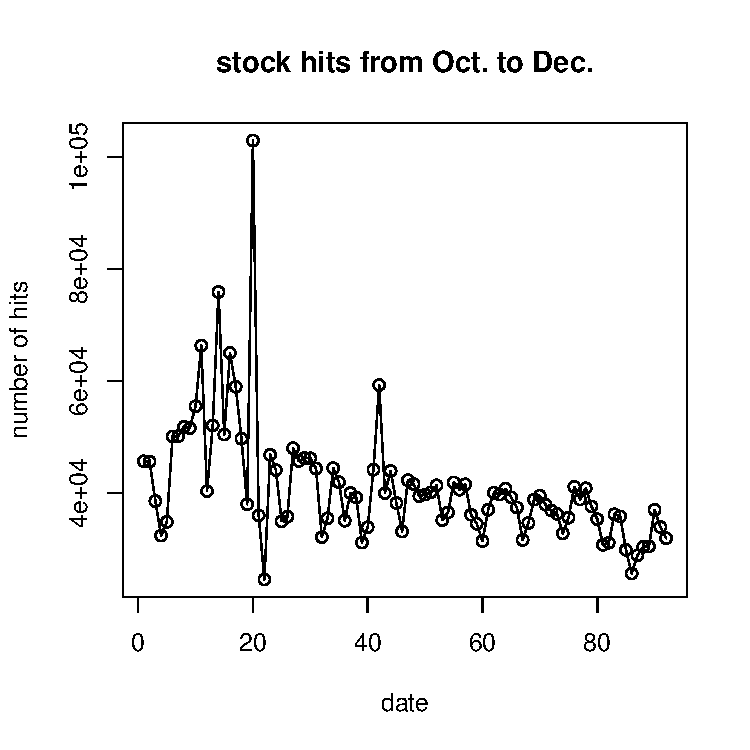
\includegraphics[width=\maxwidth]{figure/r-chunk3-1} 

\end{knitrout}

We can find that the number of hits before 10-20 is larger that those later. And 10-20 has extremely large number of hits on stock. Then I search the news and find that on that day,investors cheered comments from Federal Reserve Chairman Ben Bernanke Monday that suggested a second economic stimulus package could be up for discussion. This can explain why stock got large hits and The Dow Jones industrial average added 413 points,The Standard Poor's 500 index gained 4.8 percent and the Nasdaq composite added 3.4 percent.

But after that day, the stock market still kept going down. I guess investors did not trust the government any more and temprarily gave up the stock market, so that the number of hits on stock later was consistently small.

\section{Question4}
\subsection{(a)}

the following code is the Rscript which is run in savio.
\begin{knitrout}
\definecolor{shadecolor}{rgb}{0.969, 0.969, 0.969}\color{fgcolor}\begin{kframe}
\begin{alltt}
\hlkwd{require}\hlstd{(parallel)} \hlcom{# one of the core R packages}
\hlkwd{require}\hlstd{(doParallel)}
\hlkwd{library}\hlstd{(foreach)}
\hlkwd{library}\hlstd{(readr)}
\hlstd{nCores} \hlkwb{<-} \hlkwd{as.integer}\hlstd{(}\hlkwd{Sys.getenv}\hlstd{(}\hlstr{"SLURM_CPUS_ON_NODE"}\hlstd{))}
\hlkwd{registerDoParallel}\hlstd{(nCores)}

\hlcom{###I only do the first one quarter of the data, so let nSub equals to 240}
\hlstd{nSub} \hlkwb{<-} \hlnum{240}
\hlkwd{setwd}\hlstd{(}\hlstr{'/global/scratch/paciorek/wikistats_full/dated_for_R'}\hlstd{)}

\hlcom{###set the dir as a list of filename}
\hlstd{dir} \hlkwb{<-} \hlkwd{list.files}\hlstd{(}\hlkwc{pattern} \hlstd{=} \hlstr{"part*"}\hlstd{)}

\hlcom{###write the find function. input the directory and output the corresponding result}
\hlstd{find} \hlkwb{<-} \hlkwa{function}\hlstd{(}\hlkwc{dir}\hlstd{) \{}
  \hlstd{table} \hlkwb{=} \hlkwd{read_delim}\hlstd{(dir,} \hlkwc{delim} \hlstd{=} \hlstr{" "}\hlstd{,} \hlkwc{col_names} \hlstd{= F)}
  \hlstd{data} \hlkwb{=} \hlkwd{as.data.frame}\hlstd{(table)}
  \hlstd{row_number} \hlkwb{=} \hlkwd{grep}\hlstd{(}\hlstr{"Barack_Obama"}\hlstd{, data[,}\hlnum{4}\hlstd{])}      \hlcom{#get the row number of targeted rows}
  \hlstd{find_result} \hlkwb{<-} \hlstd{data[row_number,]}                 \hlcom{#get the result according to the row numbers}
  \hlkwd{return}\hlstd{(find_result)}
\hlstd{\}}

\hlcom{#get the final result by putting all partial result together}
\hlstd{result_final} \hlkwb{<-} \hlkwd{foreach}\hlstd{(}\hlkwc{i} \hlstd{=} \hlnum{1}\hlopt{:}\hlstd{nSub,}
                  \hlkwc{.combine} \hlstd{= rbind}
\hlstd{)} \hlopt \hlstd{\{}
  \hlstd{result_part} \hlkwb{<-} \hlkwd{find}\hlstd{(dir[i])}
  \hlstd{result_part}
\hlstd{\}}

\hlcom{###output the dimension of the final txt and the first 10 lines in the final result}
\hlstd{dim}\hlkwb{<-}\hlkwd{dim}\hlstd{(result_final)}
\hlstd{head}\hlkwb{<-}\hlkwd{head}\hlstd{(result_final,}\hlnum{10}\hlstd{)}
\hlkwd{write.table}\hlstd{(result_final,}\hlkwc{file}\hlstd{=}\hlstr{'/global/home/users/jinhui_xu/result.txt'}\hlstd{)}
\hlkwd{write.table}\hlstd{(dim,}\hlkwc{file}\hlstd{=}\hlstr{'/global/home/users/jinhui_xu/dim.txt'}\hlstd{)}
\hlkwd{write.table}\hlstd{(head,}\hlkwc{file}\hlstd{=}\hlstr{'/global/home/users/jinhui_xu/head.txt'}\hlstd{)}
\end{alltt}
\end{kframe}
\end{knitrout}

Run .sh in savio to get the result
\begin{knitrout}
\definecolor{shadecolor}{rgb}{0.969, 0.969, 0.969}\color{fgcolor}\begin{kframe}
\begin{alltt}
sbatch ps6_q4.sh
\end{alltt}
\end{kframe}
\end{knitrout}

Then I copy the txt file to my mac.
\begin{knitrout}
\definecolor{shadecolor}{rgb}{0.969, 0.969, 0.969}\color{fgcolor}\begin{kframe}
\begin{alltt}
scp jinhui_xu@dtn.brc.berkeley.edu:~/dim.txt ~/stat243/stat243-fall-2017/myps/stat243/ps6
scp jinhui_xu@dtn.brc.berkeley.edu:~/head.txt ~/stat243/stat243-fall-2017/myps/stat243/ps6
\end{alltt}
\end{kframe}
\end{knitrout}

Show the result in R. As the second lines of the result is too long, I don't show it.
\begin{knitrout}
\definecolor{shadecolor}{rgb}{0.969, 0.969, 0.969}\color{fgcolor}\begin{kframe}
\begin{alltt}
\hlkwd{read.csv}\hlstd{(}\hlstr{'~/stat243/stat243-fall-2017/myps/stat243/ps6/dim.txt'}\hlstd{)}
\end{alltt}
\begin{verbatim}
##          x
## 1 1 108833
## 2      2 6
\end{verbatim}
\begin{alltt}
\hlkwd{read.csv}\hlstd{(}\hlstr{'~/stat243/stat243-fall-2017/myps/stat243/ps6/head.txt'}\hlstd{)[}\hlkwd{c}\hlstd{(}\hlnum{1}\hlstd{,}\hlkwd{seq}\hlstd{(}\hlnum{3}\hlstd{,}\hlnum{10}\hlstd{)),]}
\end{alltt}
\begin{verbatim}
## [1] 14046 20081129 210000 pt Barack_Obama 86 2032215                                                                       
## [2] 77377 20081108 190000 no Bilde:Barack_Obama_2004.jpg 1 7825                                                            
## [3] 90408 20081128 190001 en Early_life_and_career_of_Barack_Obama 16 760462                                               
## [4] 117199 20081110 160000 et Barack_Obama 4 55875                                                                         
## [5] 160067 20081101 110000 fr Discuter:Barack_Obama 1 20922                                                                
## [6] 160311 20081205 230000 en Image:20081102_Bruce_Springsteen_and_Barack_Obama_hug.JPG 2 18562                            
## [7] 163170 20081114 210000 en Barack_Obama_Senior 1 17687                                                                  
## [8] 190861 20081107 020000 de.n Barack_Obama_will_auf_staatliche_Zusch%C3%BCsse_f%C3%BCr_seinen_Wahlkampf_verzichten 1 8656
## [9] 228377 20081008 090001 commons.m Image:Barack_Obama_and_supporters_5,_February_4,_2008.jpg 2 11675                     
## 10 Levels: 117199 20081110 160000 et Barack_Obama 4 55875 ...
\end{verbatim}
\end{kframe}
\end{knitrout}
We can see that the row number of the result is 108833. Because I only search in a quarter of files, the total number roughly equals to 430000. 

\subsection{(b)}
Copy the .out file to my mac
\begin{knitrout}
\definecolor{shadecolor}{rgb}{0.969, 0.969, 0.969}\color{fgcolor}\begin{kframe}
\begin{alltt}
scp jinhui_xu@dtn.brc.berkeley.edu:~/ps6_q4.out ~/stat243/stat243-fall-2017/myps/stat243/ps6
\end{alltt}
\end{kframe}
\end{knitrout}

Then see the time used. It used about 23min to process one quarter of files. So if I run my code on 4 times as many cores, I need about 23min to process all files. 
Therefore, I think it takes much less time to run the spark code. About 15min vs 23min.
\begin{knitrout}
\definecolor{shadecolor}{rgb}{0.969, 0.969, 0.969}\color{fgcolor}\begin{kframe}
\begin{alltt}
\hlstd{out}\hlkwb{<-}\hlkwd{readLines}\hlstd{(}\hlstr{'ps6_q4.out'}\hlstd{)}
\hlstd{out[}\hlkwd{c}\hlstd{(}\hlkwd{length}\hlstd{(out)}\hlopt{-}\hlnum{1}\hlstd{,}\hlkwd{length}\hlstd{(out))]}
\end{alltt}
\begin{verbatim}
## [1] "     user    system   elapsed " "12527.490 10420.614  1431.118 "
\end{verbatim}
\end{kframe}
\end{knitrout}

\section{Question5}
\subsection{(a)}
First, we look at the algorithm for computing U:\\

1.$U_{11}=\sqrt{A_{11}}$\\

2.For $j=2,...,n,U_{1j}=A_{1j}/U_{11}$\\

3.For $i=2,...,n,$
$$U_{ii}=\sqrt{A_{ii}-\sum_{k=1}^{i-1}U_{ki}^{2}}$$
$$for \ \ j=i+1,...,n:\ U_{ij}=({A_{ij}-\sum_{k=1}^{i-1}U_{ki}U_{kj})/U_{ii}$$

Then obviously, the operation count equals to n-1 when calculate the 1st row of U, and equals to $[i-1+(n-i)i]$ when calculate the ith row of U. Therefore the total operation count N equals to 
$$N=\sum_{i=1}^{n}[i-1+(n-i)i]=(n^{3}+3n^{2}-4n)/6$$

\subsection{(b)}
Yes, we can store the Cholesky upper triangular matrix in the block of memory that is used for the original matrix.\\
According to the algorithm in the section {(a)}, we know that we calculate $U_{ij}$ from left to right, and from up to down. In this way, we do not need the value of $A_{xy}$ where $x<i,y<j$when we calculate $U_{ij}$. Threfore, we can store $U_{ij}$ into the place of $A_{ij}$.

\end{document}
